\documentclass[12pt]{article}

\usepackage{sbc-template}

\usepackage{indentfirst}

\usepackage{graphicx,url}

\usepackage[brazil]{babel}   
  
\usepackage[utf8]{inputenc}  
% UTF-8 encoding is recommended by ShareLaTex
\usepackage{ amssymb }     
     
\sloppy

\title{Relatório de Implementação de Projeto Prático com uma Árvore com Números Variados de Filhos}
\author{Gislainy Crisostomo Velasco}
\address{Instituto de Informática – Universidade Federal de Goiás (UFG)\\
Caixa Postal 131 –- 74001-970  –- Goiânia –- GO -– Brasil
\email{gislainycrisostomo@gmail.com}
}

\begin{document} 

\maketitle

\begin{abstract}
  This extended summary presents a solution to a problem with the URI Online Judge platform. The proposed solution uses the Tree with Varied Numbers of Children. This work discusses the solution adopted, its complexity, as well as the test cases and the results obtained according to the instances.
\end{abstract}
     
\begin{resumo} 
Este resumo estendido apresenta solução de um problema da plataforma URI Online Judge. A solução proposta utiliza da Árvore com Números Variados de Filhos. Neste trabalho é discutido a solução adotada, sua complexidade, bem como os casos de testes e os resultados obtidos de acordo com as instâncias. 
\end{resumo}

\section{Introdução}

Em Ciência da Computação tradicionalmente são utilizadas abstrações do mundo real para resolver problemas computacionais. Um exemplo é a estrutura de dados árvore que se assemelha a estrutura física de uma árvore encontrada na natureza, pois existe uma relação estrutural entre seus elementos e sua organização. Nesse sentindo, ao longo do tempo foram propostas vários algoritmos de árvores que possibilitaram armazenar e manipular os dados com eficácia e eficiência. 

Usualmente são utilizados árvores que possuem como característica um número predefinidos de filhos e também uma relação de organização dos seus dados. Nesse sentido, tem se a Árvore Binária, uma estrutura conhecida e diversos outros algoritmos utiliza seus princípios como base, nela todos os nós a esquerda são menores que a raiz e a direita, maiores \cite{cormen2009introduction}. Com isso, caso for necessário a representação de uma árvore da forma que 
é encontrada na natureza, um galho pode possuir de 0 a N filhos, sem conhecimento do valor máximo de filhos, é necessário a utilização de outra estrutura de dados que permita armazenar um número variados de filhos por nós.

Dado esse cenário, este trabalho tem como propósito a implementação de um algoritmo que tem como principio o armazenamento de número variado de filhos para um determinado nó. O problema proposto foi extraído da plataforma URI Online Judge\footnote{https://www.urionlinejudge.com.br/judge/pt/problems/view/2575}. O algoritmo e testes realizados foram feitos em um contexto acadêmico, proposto e supervisionado pelos professores da disciplina Análise de Dados e Projeto de Algoritmos, de um Programa de Pós Graduação em Ciência da Computação.

Este artigo está dividido da seguinte forma: a Seção \ref{sec:definicoes} apresenta os Conceitos Básicos; a Seção \ref{sec:problema} apresenta a Descrição do Problema bem como suas entradas e saídas; a Seção \ref{sec:solucao} discorre sobre a Solução Adotada, bem como fluxo do algoritmo implementado e sua complexidade; a Seção \ref{sec:casosdeteste} apresenta os Casos de Testes realizados, comportamento do algoritmo de acordo com as entradas e suas possíveis saídas, além de apresentar as Instâncias e Resultados; por fim, a Seção \ref{sec:conclusão} apresenta a Conclusão.

\section{Conceitos Básicos}\label{sec:definicoes}

Árvore é uma estrutura de dados extremamente importante em Ciência da Computação, na qual possui uma relação estrutural entre seus dados, denominados de nós, sendo uma relação de hierarquia, onde um conjunto de nós são hierarquicamente subordinados a outro \cite{monard1993tecnicas}. Formalmente, uma árvore é um conjunto finito de um ou mais nós onde:  
\begin{enumerate}
    \item existe um nó especial denominado raiz da árvore; 
    \item os demais nós formam n conjuntos disjuntos (n $>$ 0), onde cada um destes conjuntos T (1 $<$ i $<$ n) é, por sua vez, uma árvore. As árvores T, são chamadas de subárvores da raiz. 
\end{enumerate}

Nesse contexto, existem inúmeras representações dessa estrutura, como a Árvore Binária, AVL, Rubro Negro, \textit{Heapsort}. As abordagens citadas possuem em comum que existe um número predefinido de filhos para cada nó \cite{cormen2009introduction}. Não sendo possível representar uma estrutura de dados que não se tem conhecimento de quantos filhos um nó pode ter. Nesse sentido, para representar uma árvore com um número variados de filhos, Figura \ref{fig:arvore-n-filhos}, os filhos de um nó são representados por uma lista, onde:

\begin{enumerate}
    \item um nó aponta para o seu primeiro filho;
    \item cada filho aponta para o próximo irmão.
\end{enumerate}

\begin{figure}[ht]
\centering
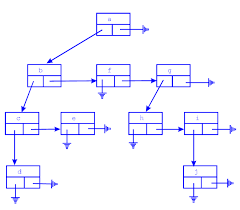
\includegraphics[width=.5\textwidth]{arvore-n-filhos.png}
\caption{Representação de uma árvore com número variados de filhos}
\label{fig:arvore-n-filhos}
\end{figure}

\section{Descrição do problema}\label{sec:problema}

O problema foi extraído da plataforma URI Online Judge. É apresentado uma história na qual o personagem principal realiza cortes em uma árvore de natal. Para realizar tal operação, é definido o critério de beleza do galho, os valores negativos representam que o galho é feio. A beleza final da árvore é dada pela soma das belezas de seus galhos. 

O método de poda tradicional que não utiliza nenhum critério de otimização é apresentado na Figura \ref{fig:2575_a}. Quando um galho é removido, todos os galhos filhos são removidos também. Na árvore à direita, os galhos cortados estão pontilhados, enquanto os nós e galhos que caíram após o corte estão tracejados. Neste exemplo, tanto a árvore sem corte, quanto a cortada possuem um valor 10 de beleza.

\begin{figure}[ht]
\centering
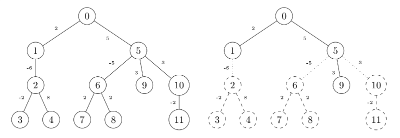
\includegraphics[width=.5\textwidth]{2575_a.png}
\caption{Corte sem critério}
\label{fig:2575_a}
\end{figure}

O método proposto utilizando critério de otimização, no qual é realizado o menor número de cortes para obter o maior grau de beleza da árvore é apresentado na Figura \ref{fig:2575_b}.

\begin{figure}[ht]
\centering
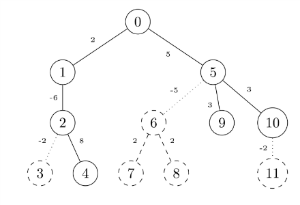
\includegraphics[width=.5\textwidth]{2575_b.png}
\caption{Corte ótimo}
\label{fig:2575_b}
\end{figure}


\subsection{Entrada}

A entrada consiste de um inteiro \textbf{N} (2 $<$ \textbf{N} $<$ $2^{6}$) que é a quantidade de nós da árvore. Nas próximas \textbf{N}-1 linhas, temos quatro inteiros \textbf{di} (0 $<$ di $<$ N-2), \textbf{ai} (0 $<$ ai $<$ \textbf{N}-1), \textbf{bi} (0 $<$ \textbf{bi} $<$ N-1),  e \textbf{wi}  (-1000 $<$ \textbf{wi} $<$ 1000) representando o identificador do galho \textbf{i}, que ele conecta o nó \textbf{ai} ao nó \textbf{bi}, e que ele possui \textbf{wi} de beleza pela classificação de Roberto. A árvore é sempre enraizada no nó 0. É garantido que o grafo da entrada é conexo e não possui ciclos.

\subsection{Saída}

A saída deve conter dois inteiros, D e M que representam o quão bonito é a árvore com o corte ótimo e quantos cortes precisam ser feitos, respectivamente. Se o número de cortes for maior do que 0, na próxima linha, imprima M inteiros \textbf{dj} em ordem crescente e separados por espaço, onde \textbf{dj} representa o identificador de cada galho \textbf{j} a ser cortado.

Caso exista mais de uma árvore com o mesmo grau de beleza, imprima aquela que possui menos galhos. Se ainda existir mais de uma árvore que satisfaça os mesmos critérios, imprima a que possua menos cortes.

\section{Solução adotada}\label{sec:solucao}

A estrutura de dados escolhida para a solução\footnote{https://github.com/gislainy/2575-Christmas-Tree} do problema foi a árvore com números variados de filhos não balanceada na qual foi adicionado além do valor do elemento, a referência do primeiro e próximo, a referência do nó pai, a beleza e uma variável de controle para remoção.

Toda a árvore é enraizada do nó 0, sendo assim, quando é realizada uma entrada é feito uma pesquisa em toda a árvore para encontrar a posição que do elemento a ser inserido, no pior caso é percorrido toda a estrutura. Dessa forma, para N-1 inserções é realizada $\sum_{n=0}^{n-1} i*n$ operações de busca para o pior caso, com complexidade O(${n^2}$). Entradas inválidas são descartadas na inserção. Os  nós folhas com beleza negativas são marcadas para remoção no momento da inserção.


Após o processo de inserção, é realizado uma busca na árvore por todos os nós que possuem valor de beleza menor igual a zero e armazenados em uma lista, sua complexidade é O(n). Para cada elemento da lista, é realizado um cálculo da beleza dos nós filhos desta subárvore, caso for menor igual a zero, todos os nós dessa subárvore são marcados para remoção. 

Após esse processamento, é calculado a beleza final da árvore e apresentado os identificadores dos galhos que de menor profundidade que foi marcado para remoção, pois quando um galho é removido todos os seus dependentes são removidos automaticamente. 

São removidos as subárvores com beleza igual a zero, pois há uma restrição do problema que se existir mais de uma árvore com o mesmo grau de beleza apresentar a que possui menos galhos. 

\section{Casos de Testes}\label{sec:casosdeteste}
Foram realizados diversos testes sendo observados 4 saídas possíveis de acordo com as instâncias.
\begin{enumerate}
    \item Não existe nó a ser removido, a beleza da árvore é a somatória de todos os nós;
    \item A somatória da beleza da árvore é menor ou igual a zero, logo o nó a ser removido é a raiz.
    \item Existe um ou mais nós a ser removido e a beleza da árvore é maior que zero;
    \item Existe mais de uma árvore com o mesmo grau de beleza, apresentar aquela que possui menos galhos. Se ainda existir mais de uma árvore que satisfaça os mesmos critérios, imprima a que possua menos cortes.
\end{enumerate}

\subsection{Instâncias e Resultados}

Para cada saída, foram construídas 5 instâncias de teste, com entradas de N variando 2, 10, 100, 1000 e 10000. Todos os resultados apresentados corresponderam com os resultados apresentados no uDebug\footnote{https://www.udebug.com/URI/2575}. 

As instâncias com N igual a 2, obtiveram somente dois resultados, para a saída 2 foi apresentado que havia uma remoção e grau de beleza 0 e, para todos os outros resultados o grau beleza máxima da árvore sem nenhum corte.

Para as saídas 1 e 2, todas as instâncias tiveram os resultados esperados, no caso 2, todas as saídas foram que havia grau de beleza 0 e o nó a ser removido era a raiz. No caso da saída 1, quanto maior o N, maior o número de nós a ser removido e consequentemente o grau de beleza.

No caso 4, foram construídas instâncias com o grau de filhos para cada nó igual a 10. Foram criadas 8 instâncias de testes, sendo 2 grupos de 4 instâncias, sendo um grupo com os galhos pares com grau de beleza positivo e ímpar negativo e o outro grupo o inverso. Para todos os testes, foi observado que os números de galhos a ser removidos correspondiam a 45\% dos galhos totais da árvore.


\section{Conclusões}\label{sec:conclusão}

A solução adotada atende os critérios estabelecidos para o problema proposto. O fato de não possui um conhecimento prévio de como os dados estão organizados traz uma complexidade maior ao realizar operações de busca e inserção, além das operações que foram inseridas para solucionar o problema, como a função de calcular os nós que serão removidos e cálculo da beleza da árvore resultante. 

A árvore com um número variados de filhos não balanceada deve somente ser utilizada quando realmente não se sabe um número máximo de filhos que um nó pode ter, pois, quando maior a fica ao longo do tempo, maior o número de comparação para inserção e também exige maior controle para remoção de um determinado nó.

\bibliographystyle{sbc}
\bibliography{sbc-template}

\end{document}
